\chapter{Physics and Measurement Models in Emission Tomography}
\label{chap:intro_material}

This chapter introduces the physical principles and measurement models underpinning emission tomography, with emphasis on the effects that dominate reconstruction quality and quantitative reliability. In both \acrfull{pet} and \acrfull{spect}, the reconstruction task is to infer a non-negative radiotracer activity distribution from projection data generated by stochastic radioactive decay and corrupted by attenuation, scatter, and blurring effects. These are naturally captured by a forward model that maps the image to expected measurement counts with additive components representing background contributions.

We first summarise the detection physics of \gls{pet} and \gls{spect} and present convenient factorisations of the system matrix that separate geometry, attenuation, and detector effects. We then focus on the particularly challenging case of post-\gls{sirt} \gls{y90} imaging, where quantification is limited by extreme count starvation in \acrfull{ipp} \gls{pet} and by spectral and resolution degradations in bremsstrahlung \gls{spect}. Finally, we describe the role of \acrfull{ct} in this thesis as the source of attenuation information required for physically accurate emission modelling and a high-resolution anatomical reference for reconstruction regularisation in low-count regimes.

\section{Principles of Emission Tomography}

\gls{pet} fundamentally differs from anatomical modalities such as \gls{ct}. Rather than mapping the structural properties, \gls{et} measures the spatio-temporal distribution of a radiolabelled substance introduced into the physiological system. A representative example is \gls{fdg}\cite{boellaardFDGPETCT2015}. \gls{fdg} is a glucose-analogue, meaning energy-hungry cells take up an increased amount of the molecules, and therefore radionuclide. Cells are unable to metabolise \gls{fdg}, meaning it accumulates. The distribution of \gls{fdg} can be imaged using a \gls{pet} scanner, giving a functional view of glucose metabolism and highlighting any unusual uptake caused by overactive cells such as cancer.

While the instrumentation differs between \gls{spect} and \gls{pet}, both involve a similar inverse problem: estimating the activity distribution from projection measurements governed by Poisson counting statistics, attenuation, scatter, and detector resolution. The continuous activity distribution is represented on a finite voxel grid as a non-negative image vector $x\in\mathbb{R}_+^J$. The primary contribution to the expected measurements is modelled using the non-negative system matrix $A\in\mathbb{R}_+^{I\times J}$. Including additive background contributions gives the affine forward model
\begin{equation}
\bar{y}=Ax+b,
\end{equation}
where $\bar{y}=\mathbb{E}[y]\in\mathbb{R}_+^I$ denotes the total expected measurement counts and $b\in\mathbb{R}_+^I$ contains contributions not described by the primary emission model. The precise discretisation and statistical measurement model are introduced later.

\section{Positron Emission Tomography (\gls{pet})}\label{sec:pet}

\gls{pet} primarily uses neutron-deficient isotopes (see Section~\ref{sec:y90} for a counter-example)  that stabilise via $\beta^+$ decay. Within the nucleus, a proton converts into a neutron, emitting a positron ($e^+$) and an electron neutrino ($\nu_e$) to conserve lepton number:
\begin{equation}
    p \rightarrow n + e^+ + \nu_e.
\end{equation}
The decay energy is shared between the positron and the neutrino, resulting in a continuous positron energy spectrum. This positron traverses the tissue losing kinetic energy via Coulomb interactions (a distance known as the positron range) before thermalising. This range imposes an effective blurring limit on spatial resolution, with an effective positron range of approximately 0.5–0.7 mm for $^{18}$F and several millimetres for high-energy emitters such as $^{82}$Rb \cite{cherryPhysicsNuclearMedicine2003}.

Upon thermalisation, the positron interacts with an electron to form positronium, which rapidly decays via annihilation:
\begin{equation}
    e^+ + e^- \rightarrow \gamma + \gamma
\end{equation}
The rest mass energy of the pair ($2 \times 511$ keV) is converted into two\footnote{Positron/electron pairs can also annihilate to produce more than two photons but this is much less likely ($p(3\gamma)/p(2\gamma)\approx$1/378)\cite{bass_colloquium_2023}} (near) anti-parallel\footnote{In order to conserve momentum, a certain a-collinearity will exist between the photons, introducing additional blurring \cite{shibuyaAnnihilationPhotonAcollinearity2007}.} photons (Figure~\ref{fig:positron_annihilation}).

\begin{figure}
    \centering
    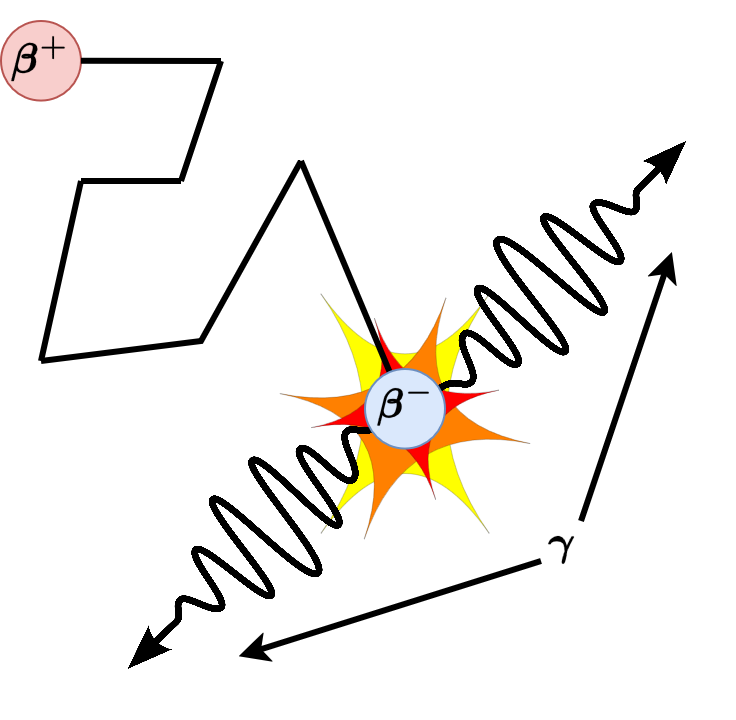
\includegraphics[width=0.7\linewidth]{figures/Chapter1/proton_annihilation.drawio.png}
    \caption{A positron traverses tissue, losing kinetric energy, before annihilating with an electron, resulting in two (nearly) anti-parallel photons.}
    \label{fig:positron_annihilation}
\end{figure}

\subsection{Coincidence Detection and Data Acquisition}\label{subsec:pet:acquisition}

\gls{pet} detectors are typically assembled into modular detector blocks, which are then arranged circumferentially to form a ring around the patient. Modern clinical systems comprise multiple such rings stacked along the axial direction, increasing axial coverage and sensitivity by enlarging the axial \gls{fov}. Figure~\ref{fig:pet_rings} illustrates this geometry showing a single ring in the axial view, and multiple rings in the sagittal view.

%Really shite quality images. Shoudl delete. Not sure if Ir eall need these, anyway
\begin{figure*}[t!]
    \centering
    \begin{subfigure}[t]{0.5\linewidth}
        \centering
        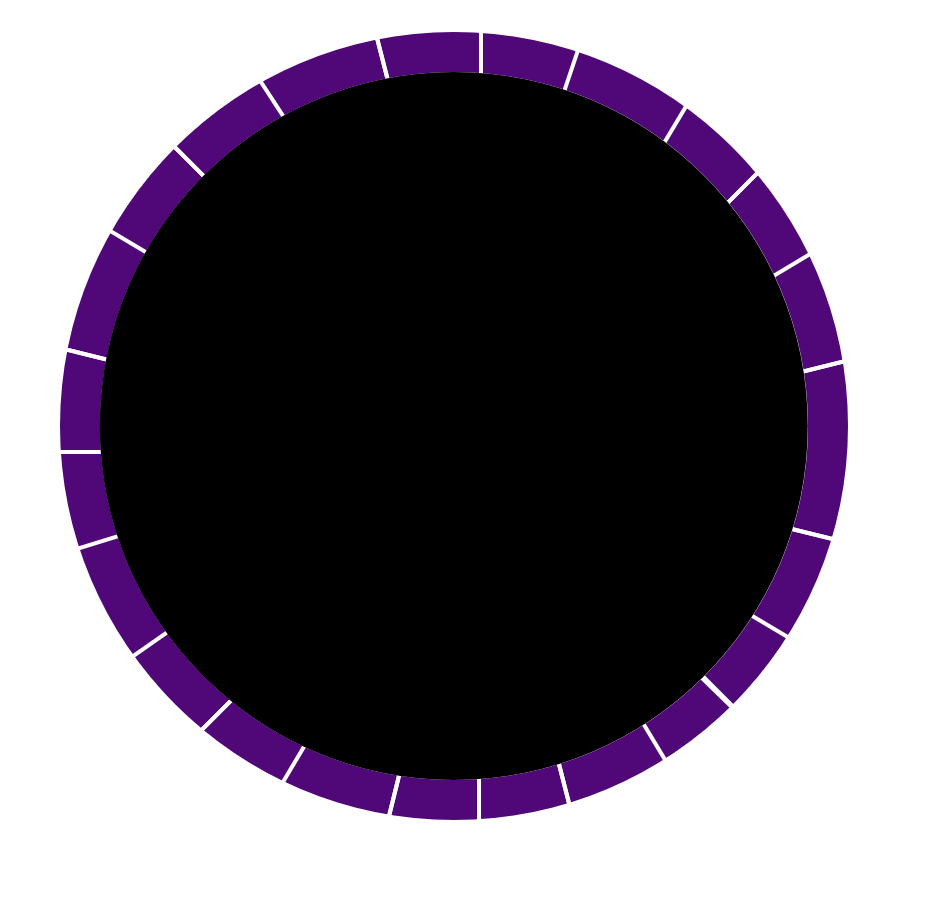
\includegraphics[width=\linewidth]{figures/Chapter1/PET_axial.drawio.png}
        \label{subfig:pet_rings_axial}
    \end{subfigure}%
    \hspace{2cm}
    \begin{subfigure}[t]{0.12\linewidth}
        \centering
        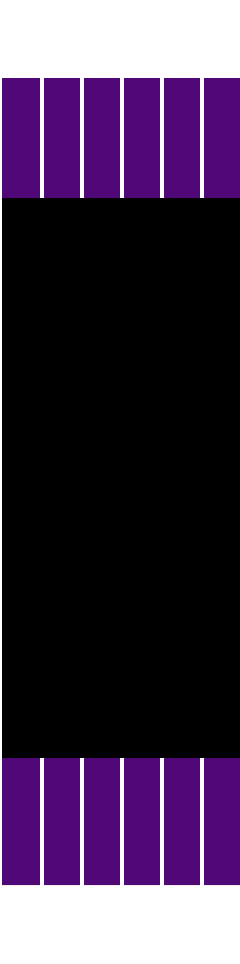
\includegraphics[width=\linewidth]{figures/Chapter1/PET_sagittal.drawio.png}
        \label{subfig:pet_rings_sagittal}
    \end{subfigure}
    \caption{Simple diagram of a \gls{pet} scanner. Left, axial view showing detectors arranged in a ring. Right, sagittal/coronal view showing multiple rings forming the axial \glsentryshort{fov}.}
\label{fig:pet_rings}
\end{figure*}

\gls{pet} imaging relies on a technique known as electronic collimation. A valid event is recorded only if two detectors register photons within a coincidence timing window $2\tau$ (typically 6--12 ns) \cite{cherryPhysicsNuclearMedicine2003}. The measured coincidences (or counts) along a \gls{lor}, connecting detectors $1$ and $2$, denoted as $y_{i_{1,2}}$, is a superposition of three components:
\begin{equation}
    y_{i_{1,2}} = t_{i_{1,2}} + s_{i_{1,2}} + r_{i_{1,2}}
\end{equation}
where $t_{ij}$ represents true coincidences (Figure~\ref{subfig:pet_true_scatter}, right), $s_{i_{1,2}}$ represents scatter (where one or both photons have undergone at least one Compton interaction; Figure~\ref{subfig:pet_true_scatter}, left)), and $r_{i_{1,2}}$ represents random coincidences (Figure~\ref{subfig:pet_randoms}).

\begin{figure*}[t!]
    \centering
    \begin{subfigure}[t]{0.5\linewidth}
        \centering
        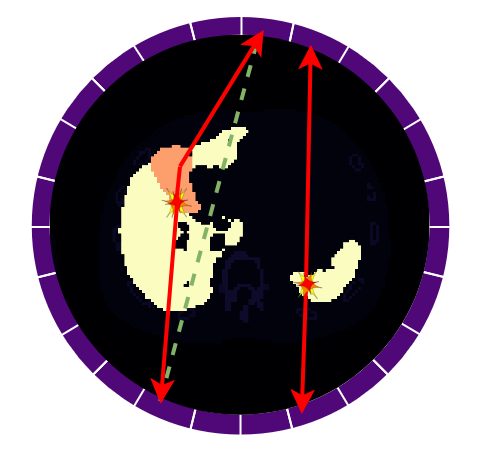
\includegraphics[width=\linewidth]{figures/Chapter1/PET_diagram.drawio.png}
        \caption{}
        \label{subfig:pet_true_scatter}
    \end{subfigure}%
    ~ 
    \begin{subfigure}[t]{0.5\linewidth}
        \centering
        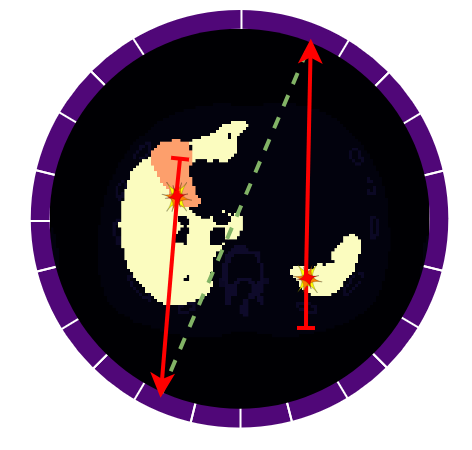
\includegraphics[width=\linewidth]{figures/Chapter1/PET_rand_diagram.drawio.png}
        \caption{}
        \label{subfig:pet_randoms}
    \end{subfigure}
    \caption{Possible coincidences under \gls{pet} electronic collimation. Panel (a) shows a scattered coincidence (the green dashed line is the effective \gls{lor}) and a true coincidence; panel (b) shows a random coincidence (green dashed lines are the effective \glspl{lor}).}
\label{fig:pet}
\end{figure*}

Random coincidences occur when two unrelated annihilation events are detected within the timing window. The rate of randoms on a specific \gls{lor} is governed by the singles rates of the individual detectors ($R_1, R_2$), often approximated as:
\begin{equation}
    r_{i_{1,2}} = 2\tau R_1 R_2.
\end{equation}

\subsection{The \gls{pet} model}\label{subsec:pet:model}
\label{sec:pet_model}

In \gls{pet}, the system matrix may be factorised as
\begin{equation}
    A = A_{\mathrm{det,sens}}\,A_{\mathrm{det,blur}}\,A_{\mathrm{att}}\,A_{\mathrm{geom}}\,A_{\mathrm{ToF}}\,A_{\mathrm{positron}}.
\end{equation}
Here, $A_{\mathrm{positron}}$ models positron-range blurring, $A_{\mathrm{ToF}}$ models the timing localisation accuracy for \gls{tof} \gls{pet} (and is omitted for non-\gls{tof} \gls{pet}), $A_{\mathrm{geom}}$ is the geometric projection operator mapping voxels to lines of response in the absence of attenuation, $A_{\mathrm{att}}$ is a diagonal operator containing attenuation factors along each line of response, $A_{\mathrm{det,blur}}$ models detector-related resolution effects in reporting the true line-of-response positions, and $A_{\mathrm{det,sens}}$ is a diagonal sensitivity factor incorporating multiplicative effects such as detector efficiencies and normalisation \cite{baileyNuclearMedicinePhysics2014a}. The additive term is commonly written as $b=s+r$, corresponding to scatter and randoms, respectively.

\section{Single Photon Emission Computed Tomography (\gls{spect})}

\Gls{spect} imaging relies on single gamma emissions. As there is no coincident pair to define the \gls{lor}, physical collimation is required. A lead collimator, typically a parallel-hole geometry, allows only photons travelling through the collimator holes. A single (or multiple, most often a dual-head system) collimated gamma camera is rotated around the patient (Figure~\ref{fig:spect}).

\begin{figure}
    \centering
    \makebox[0pt][c]{\hspace*{-3.5cm}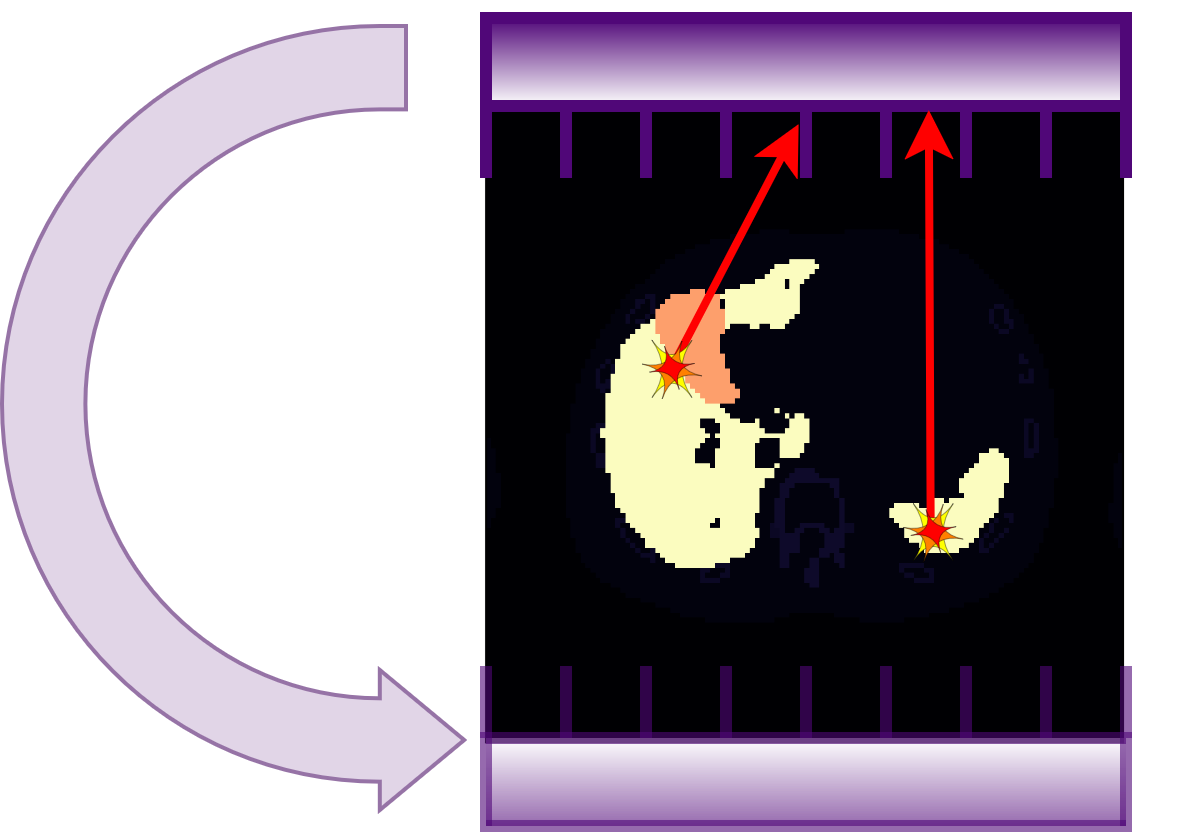
\includegraphics[width=0.7\textwidth]{figures/Chapter1/SPECT_diagram.drawio.png}}
    \caption{Left, non-parallel photon rejected by physical collimation. Right, photon parallel to the collimator can be detected, giving a line of response containing the emission source.}
    \label{fig:spect}
\end{figure}

The sensitivity ($g$) of a parallel-hole collimator depends on the hole diameter ($d$), septal thickness ($t$), and the effective hole length ($L_e$). A commonly used geometric-efficiency scaling is
\begin{equation}
    g \;\propto\; \frac{d^{4}}{L_e^{2}\,(d+t)^{2}},
\end{equation}
which makes explicit the trade-off between resolution and sensitivity: reducing $d$ improves geometric resolution but decreases sensitivity \cite{cherryPhysicsNuclearMedicine2003}. In practice, the geometric efficiency of a (high-resolution) parallel-hole collimator can be very low (often $\lesssim 0.05\%$) \cite{angerScintillationCamera1958}. In the context of bremsstrahlung imaging (Section~\ref{subsec:bremss}), this low efficiency is compounded by the continuous energy spectrum of the emissions, which limits the effectiveness of standard photopeak-based energy windowing for scatter rejection.

\subsection{The \gls{spect} model}\label{subsec:spect:model}
\label{sec:spect_model}

For \gls{spect}, a convenient factorisation is
\begin{equation}
    A \;=\; A_{\mathrm{det,sens}}\,A_{\mathrm{det,blur}}\,A_{\mathrm{geom,att}}\,A_{\mathrm{bremss}},
\end{equation}
where $A_{\mathrm{det,sens}}$ collects multiplicative sensitivity factors, $A_{\mathrm{det,blur}}$ represents intrinsic resolution effects within the gamma camera, and $A_{\mathrm{geom,att}}$ is the geometric projection operator that encapsulates collimator effects (including depth-dependent resolution) together with depth- and view-dependent attenuation. The operator $A_{\mathrm{bremss}}$ is specific to bremsstrahlung \gls{spect} and models the additional blurring associated with bremsstrahlung range (discussed in Section~\ref{subsec:bremss}).

For a parallel-hole collimator, septal penetration can be incorporated via an energy-dependent effective hole length,
\begin{equation}
    L_e(E) \;=\; l \;-\; \frac{2}{\mu_{\mathrm{}}(E)},
\end{equation}
where $l$ is the physical hole length and $\mu\mathrm(E)$ is the linear attenuation coefficient of the collimator material at photon energy $E$ \cite{cherryPhysicsNuclearMedicine2003}. The combined intrinsic detector blur and collimator blur is commonly approximated by a depth-dependent Gaussian point-spread function embedded within $A_{\mathrm{geom,att}}$, with standard deviation $\sigma(h,E)$ increasing with source-to-collimator distance $h$ (and depending on $E$ through penetration).

\section{Yttrium-90 Radioembolisation (\gls{sirt})}
\label{sec:y90}

\Gls{sirt} uses \gls{y90} microspheres for the locoregional treatment of hepatic malignancies. It is an established treatment for unresectable \gls{hcc} and liver metastases \cite{sundramSelectiveInternalRadiation2017}, recommended by NICE for unresectable \glsentryshort{hcc} and used for neuroendocrine and colorectal liver metastases in the UK \cite{nationalinstituteforhealthandcareexcellenceniceSelectiveInternalRadiation2021}. NICE has since appraised radioembolisation with \isotope[166]{Ho} microspheres for the same indication \cite{nationalinstituteforhealthandcareexcellenceniceSelectiveInternalRadiation2024}, although this thesis concerns \gls{y90} throughout. The reconstruction of post-\gls{sirt} microsphere distribution presents a severe ill-posed inverse problem, as \gls{y90} is designed for therapy, not imaging.

\subsection{Decay Characteristics}
\gls{y90} is an almost pure $\beta^-$ emitter decaying to the stable ground state of \gls{zr90} with a half-life of 64.1 hours:
\begin{equation}
    ^{90}\text{Y} \rightarrow ^{90}\text{Zr} + e^- + \bar{\nu}_e
\end{equation}
The electrons have a high endpoint energy of \SI{2.28}{\mega\electronvolt}. The primary challenge for quantitative imaging is the absence of primary gamma photons. Imaging must therefore exploit two secondary, low-probability physical interactions.

\subsection{Bremsstrahlung \gls{spect}}
\label{subsec:bremss}
As high-energy $\beta^-$ particles decelerate in tissue through Coulomb interactions with charged particles, they emit Bremsstrahlung photons. These photons can be imaged with \gls{spect} systems. However, the continuous spectrum of bremsstrahlung photons (Figure~\ref{fig:brems_emission}) hugely reduces the suitability of traditional energy-window scatter-correction methods, while bremsstrahlung range blurring (Figure~\ref{fig:bremsstrahlung}) reduces resolution \cite{simpkinSpatialEnergyDependence1992}. Consequently, bremsstrahlung \gls{spect} is often characterised by poor spatial resolution and limited quantitative accuracy \cite{minarikEvaluationQuantitative90Y2008, rongDevelopmentEvaluationImproved2012}.

\begin{figure}
    \centering
    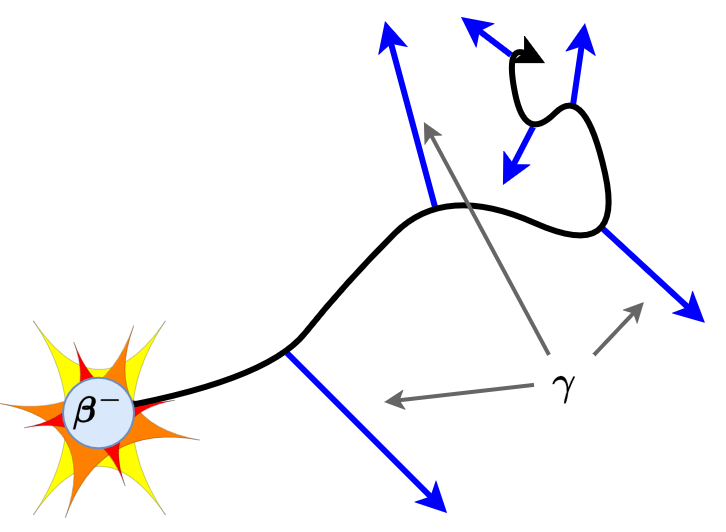
\includegraphics[width=0.5\linewidth]{figures/Chapter1/bremsstrahlung.drawio.png}
    \caption{Representative diagram of bremsstrahlung production in tissue for an emitted $\beta^{-}$ particle.}
    \label{fig:bremsstrahlung}
\end{figure}

% in preamble:
% \usepackage{subcaption}
% \usepackage{graphicx}

\begin{figure}[t]
    \centering
    \begin{subfigure}[t]{0.8\linewidth}
        \centering
        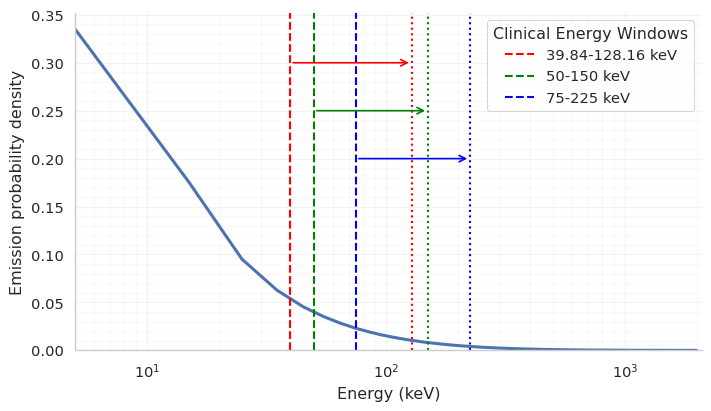
\includegraphics[width=\linewidth]{figures/Chapter1/bremsstrahlung_emission_spectrum.png}
        \caption{Bremsstrahlung emission spectrum for \gls{y90}.}
        \label{fig:brems_emission}
    \end{subfigure}
    \hfill
    \begin{subfigure}[t]{0.8\linewidth}
        \centering
        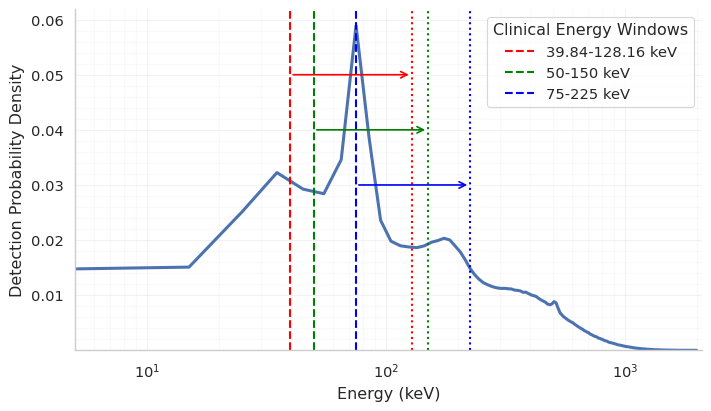
\includegraphics[width=\linewidth]{figures/Chapter1/bremsstrahlung_detected_spectrum_10cm_AnyScan.png}
        \caption{Simulated detected spectrum (10\,cm, AnyScan).}
        \label{fig:brems_detected_10cm}
    \end{subfigure}
    \caption{Bremsstrahlung spectra: (a) emitted spectrum from \gls{gate} FastY90 model \cite{raultFastSimulationYttrium902010, janGATESimulationToolkit2004} and (b) simulated detected spectra using AnyScan Trio \gls{gate} scanner model \cite{pellsQuantitativeValidationMonte2023} with a visible k-edge at $\sim$~\SI{90}{\kilo\electronvolt} resulting from photoelectric absorption in the collimator}
    \label{fig:brems_spectra}
\end{figure}


\subsection{Internal Pair Production \gls{pet}}
A minor decay branch ($31.86 \times 10^{-6}$) allows the nucleus to transition to an excited $0^+$ state of \gls{zr90}, which de-excites via \acrfull{ipp}:
\begin{equation}
    ^{90}\text{Y} \rightarrow ^{90}\text{Zr}^* + \dots \rightarrow ^{90}\text{Zr} + e^-_{IPP} + e^+_{IPP}
\end{equation}
The resulting positron annihilates to produce standard 511 keV photon pairs \cite{selwynNewInternalPair2007}. While this enables quantitative \gls{pet} imaging, the acquisition is ``count-starved'' due to the extremely low branching ratio and noise-dominated due to the Bremsstrahlung background (Figure~\ref{fig:pet_y90_profile}).

\begin{figure}
    \centering
    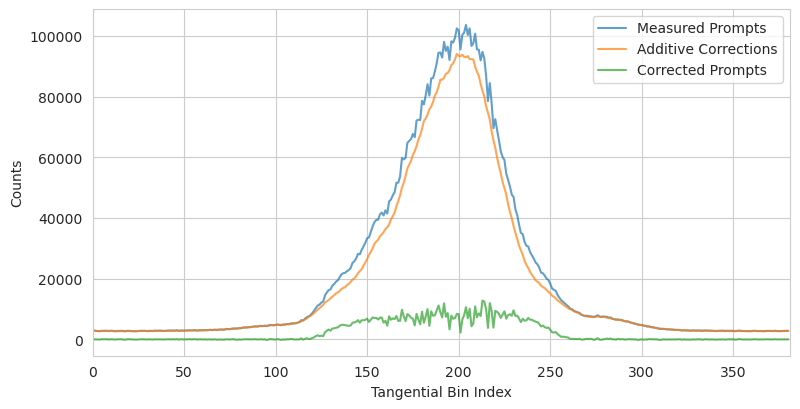
\includegraphics[width=\linewidth]{figures/Chapter1/PET_profile.png}
    \caption{Tangential profile of measured prompt counts and estimated additive terms (randoms+scatter), with the corresponding corrected prompts for an \gls{y90} \gls{pet} scan. The data are summed over all views and segments, leaving counts per tangential bin.}
    \label{fig:pet_y90_profile}
\end{figure}

\section{X-ray \gls{ct}}

In this work, \gls{ct} is used primarily to provide anatomical context and attenuation information for emission tomography reconstruction. X-ray \gls{ct} measures the transmitted intensity of a photon beam after passage through an object or patient. In an ideal monoenergetic setting, transmission follows the Beer--Lambert law, so that the log-normalised measurements are proportional to line integrals of the linear attenuation coefficient. In practice, polychromaticity introduces effects such as beam hardening, which are mitigated by scanner calibration and correction steps to yield images that approximate an attenuation map.

Reconstructed \gls{ct} images are typically reported in \gls{hu}, calibrated such that water is 0~\gls{hu} and air is $-1000$~\gls{hu}. The high spatial resolution of \gls{ct} provides structurally reliable edge information (e.g.\ liver boundaries and lesion margins) that can be used to guide regularisation in the ill-posed reconstruction of post-\gls{sirt} \gls{y90} \gls{pet} and \gls{spect}.

In addition, \gls{ct} is routinely used for \gls{ctac} in both \gls{pet} and \gls{spect}. The reconstructed \gls{hu} image is first converted to an estimate of the linear attenuation coefficient map $\mu(E)\in\mathbb{R}_+^J$ at the relevant photon energy $E$ (e.g.\ $E=$~\SI{511}{\kilo\electronvolt} for \gls{pet}, or the photopeak energy for \gls{spect}) \cite{schneider_calibration_1996, carney_method_2006}. 

Misregistration (e.g.\ respiratory motion), metal artefacts, and beam-hardening residuals can all propagate into \glsentryshort{ctac} and therefore bias quantitative \gls{pet}/\gls{spect} activity estimates \cite{singhAttenuationArtifactAttenuation2007, pattonSPECTCTPhysical2008}.
